



%%%%%%%%%%%%%%%%%%%%%%%%%%%%%%%%%%%%%%%%%%%%%%%%%%%%%%%%%%%%%%%%%%%%%%%%%%%%%%%
%%%%%%%%%%%%%%%%%%%%%%%%%%%%%%%%%%%%%%%%%%%%%%%%%%%%%%%%%%%%%%%%%%%%%%%%%%%%%%%
%%%%%%%%%%%%%%%%%%%%%%%%%%%%%%%%%%%%%%%%%%%%%%%%%%%%%%%%%%%%%%%%%%%%%%%%%%%%%%%

\chapter{The team of the Megason lab}

The Megason Lab's employee are post-doc researchers. Two domains of expertise are present : Biology and informatics.
The biology team leads researches on the development of zebra fishes,
and the computer team works on developing a program for visualization, segmentation, and tracking of cells adapted to microscopy data.

{\small \begin{tabular*}{1.0\textwidth}{@{\extracolsep{\fill}}|p{2.5cm}| p{3.cm}|p{3.5cm}|c|}
\hline Name & Status & Interest & Nationality \\ 
\hline Sean Megason & Professor & Financing and managing the laboratory. & USA \\ 
\hline Ramil Noche & Post-doctoral fellow & dynamics and function of gene regulatory networks. & Philipines \\ 
\hline Fengzhu Xiong & Graduate student & cell differentiation mechanism to create neurons and skin cell. & Chine \\ 
\hline Nikolaus Obholzer & Post-doctoral fellow  & Ear development and regeneration. &  Allemange \\ 
\hline Paul Cowgill & Graduate student & Synthetic biology, noise and development. & USA \\ 
\hline David Tulga & Graduate student & Cellular development. &  USA \\ 
\hline Ian Swiburne & Post-doctoral fellow & Ear development. & USA \\ 
\hline Andrea Tentner & Post-doctoral fellow  & Cell differentiation in spinal cord. & USA \\ 
\hline Amelia Green & Post-doctoral fellow  & Variation and regulation in organ development. & Angleterre \\ 
\hline Evan Schwab & Associate & Locations of genes responsible for mutations in the zebra fish ear using computational algorithm. & USA \\ 
\hline Dante D'India & Technicien & Animal care. & USA \\ 
\hline Arnaud Gelas & Research Engineer (senior) &  Developing {\gofigure}: Project management. &  France \\
\hline Kishore Mosaliganti & Post-doctoral fellow  & Image processing algorithms, registration and segmentation. & India \\ 
\hline Lydie Souhait & Research Engineer & Developing {\gofigure}: Responsible of the database (design, connexion, requests), and GUI & France \\
\hline Nicolas Rannou & Research Engineer &  Developing {\gofigure}: Responsible of the visualization in {\gofigure} & France \\
\hline Antonin Perrrot-Audet & Intern& Image processing : cells detection; developing {\gofigure} & France \\
\hline 
\end{tabular*} }




%%%%%%%%%%%%%%%%%%%%%%%%%%%%%%%%%%%%%%%%%%%%%%%%%%%%%%%%%%%%%%%%%%%%%%%%%%%%%%%
%%%%%%%%%%%%%%%%%%%%%%%%%%%%%%%%%%%%%%%%%%%%%%%%%%%%%%%%%%%%%%%%%%%%%%%%%%%%%%%
%%%%%%%%%%%%%%%%%%%%%%%%%%%%%%%%%%%%%%%%%%%%%%%%%%%%%%%%%%%%%%%%%%%%%%%%%%%%%%%




\chapter{Evaluation Data Illustrations}
\label{annex:EvalData}

\section{Real}

\begin{figure}[htb]
  \centering
%
\subfloat[][]{\includegraphics[width=0.3\textwidth, height=0.3\textwidth]%
{pictures/reelNucxy}\label{fig:reelNucxy}}\hspace{3pt}
%
\subfloat[][]{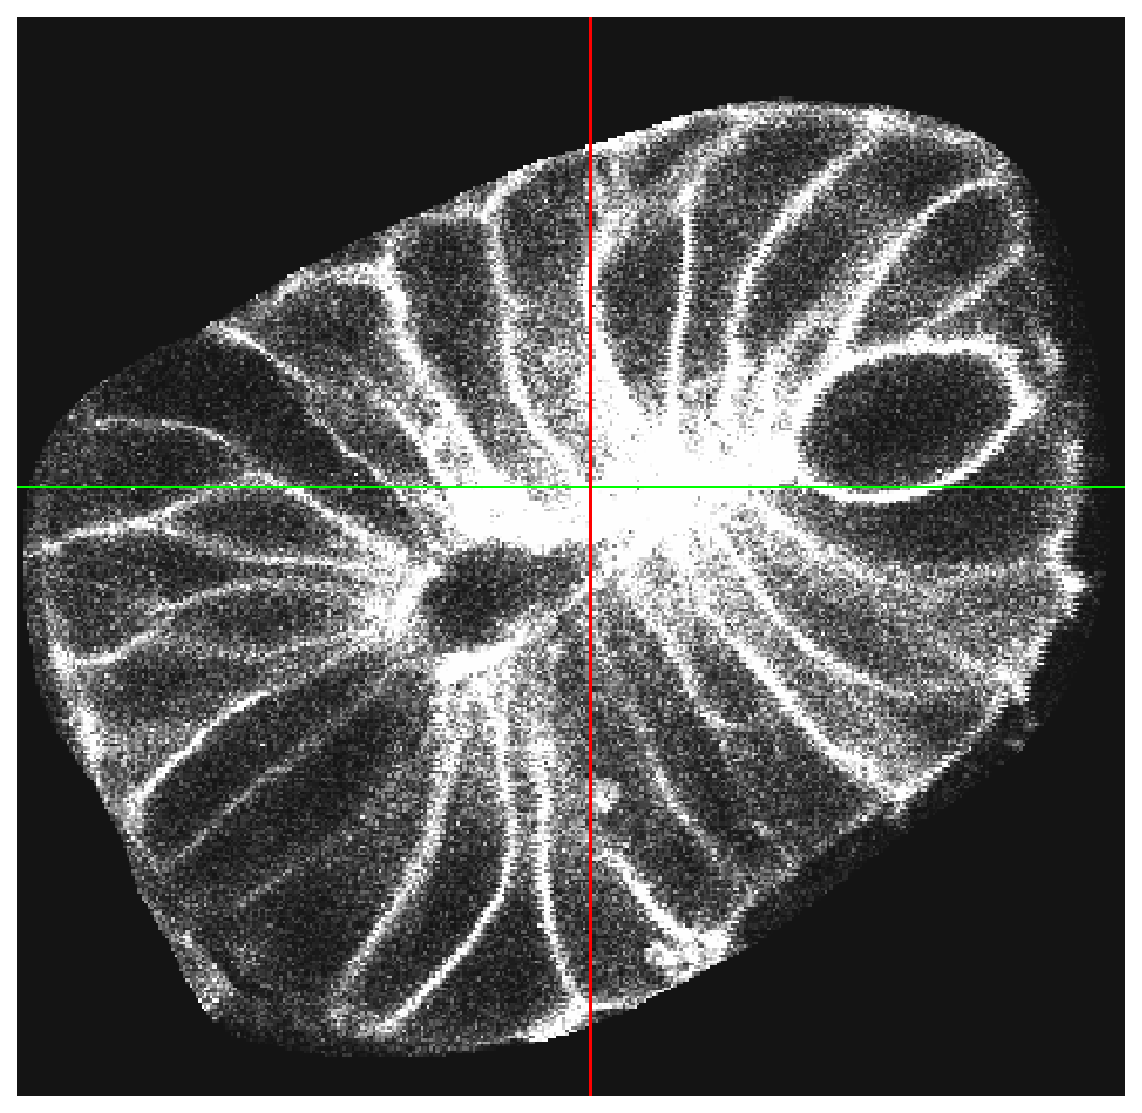
\includegraphics[width=0.3\textwidth, height=0.3\textwidth]
{pictures/reelMembxy}\label{fig:reelMembxy}}\\
%
\subfloat[][]{\includegraphics[width=0.3\textwidth, height=0.3\textwidth]%
{pictures/reelNucxz}\label{fig:reelNucxz}}\hspace{3pt}
%
\subfloat[][]{\includegraphics[width=0.3\textwidth, height=0.3\textwidth]%
{pictures/reelMembxz}\label{fig:reelMembxz}}\hspace{3pt}
%
%
%
%
%
\caption{%
xy (\subref{fig:reelNucxy},\subref{fig:reelMembxy})
 and xz (\subref{fig:reelNucxz}, \subref{fig:reelMembxz}) nuclei and corresponding membrane slices of the real dataset containing 141 cells.
}
  \label{fig:realData}
\end{figure}

\section{Synthetic}

\begin{figure}[htb]
  \centering
%
\subfloat[][]{\includegraphics[width=0.3\textwidth, height=0.29\textwidth]%
{pictures/validNuc1xy}\label{fig:validNuc1xy}}\hspace{3pt}
%
\subfloat[][]{\includegraphics[width=0.3\textwidth, height=0.29\textwidth]%
{pictures/validMemb1xy}\label{fig:validMemb1xy}}\\
%
\subfloat[][]{\includegraphics[width=0.3\textwidth, height=0.29\textwidth]%
{pictures/validNuc1yz}\label{fig:validNuc1yz}}\hspace{3pt}
%
\subfloat[][]{\includegraphics[width=0.3\textwidth, height=0.29\textwidth]%
{pictures/validMemb1yz}\label{fig:validMemb1yz}}\\
%
%
%
\subfloat[][]{\includegraphics[width=0.3\textwidth, height=0.29\textwidth]%
{pictures/validNuc10xy}\label{fig:validNuc10xy}}\hspace{3pt}
%
\subfloat[][]{\includegraphics[width=0.3\textwidth, height=0.29\textwidth]%
{pictures/validMemb10xy}\label{fig:validMemb10xy}}\\
%
\subfloat[][]{\includegraphics[width=0.3\textwidth, height=0.29\textwidth]%
{pictures/validNuc10yz}\label{fig:validNuc10yz}}\hspace{3pt}
%
\subfloat[][]{\includegraphics[width=0.3\textwidth, height=0.29\textwidth]%
{pictures/validMemb10yz}\label{fig:validMemb10yz}}\hspace{3pt}
%
%
%
%
\caption{%
xy (\subref{fig:validNuc1xy},\subref{fig:validMemb1xy})
 and yz (\subref{fig:validNuc1yz}, \subref{fig:validMemb1yz}) nuclei and corresponding membrane slices of the synthetic dataset with 100 cells and low noise.\\
xy (\subref{fig:validNuc10xy},\subref{fig:validMemb10xy})
 and yz (\subref{fig:validNuc10yz}, \subref{fig:validMemb10yz}) nuclei and corresponding membrane slices of the synthetic dataset with 1000 cells and high noise. Note that the cell volume is also smaller.
}
  \label{fig:simuData}
\end{figure}






%%%%%%%%%%%%%%%%%%%%%%%%%%%%%%%%%%%%%%%%%%%%%%%%%%%%%%%%%%%%%%%%%%%%%%%%%%%%%%%
%%%%%%%%%%%%%%%%%%%%%%%%%%%%%%%%%%%%%%%%%%%%%%%%%%%%%%%%%%%%%%%%%%%%%%%%%%%%%%%
%%%%%%%%%%%%%%%%%%%%%%%%%%%%%%%%%%%%%%%%%%%%%%%%%%%%%%%%%%%%%%%%%%%%%%%%%%%%%%%





\chapter{Detailed Evaluation Results}
\label{annex:Eval}

\section{Real Data}
\begin{figure}[H]
  \centering
  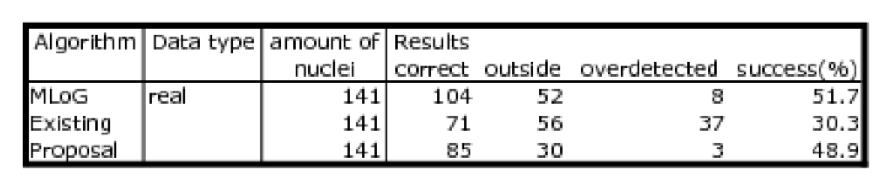
\includegraphics[width=1\textwidth]{pictures/evalReal}          
  \caption{Raw data from the evaluation framework. Processed data is a dataset from the ear of a zebrafish embryo.}
  \label{tab:realEvalRaw}
\end{figure}

This annex presents the raw results from the evaluation both on synthetic and real data of the existing algorithm in the Megason lab, the scale constrained Laplacien of Gaussian, and the proposed algorithm.
\section{Synthetic Data}
\begin{figure}[H]
  \centering
  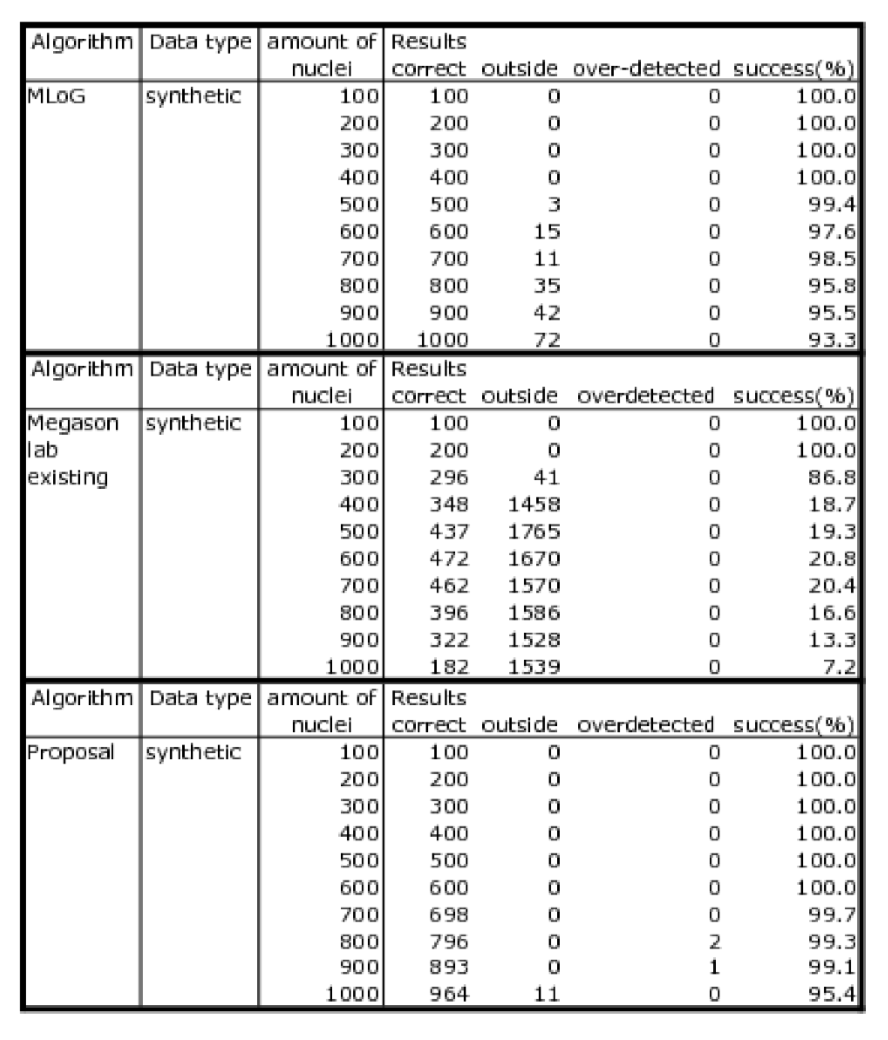
\includegraphics[width=1\textwidth]{pictures/evalTest}          
  \caption{Raw data from the evaluation framework. Processed data are 10 synthetic datasets with increasing number of nuclei and amount of noise.}
  \label{tab:syntheEvalRaw}
\end{figure}





%%%%%%%%%%%%%%%%%%%%%%%%%%%%%%%%%%%%%%%%%%%%%%%%%%%%%%%%%%%%%%%%%%%%%%%%%%%%%%%
%%%%%%%%%%%%%%%%%%%%%%%%%%%%%%%%%%%%%%%%%%%%%%%%%%%%%%%%%%%%%%%%%%%%%%%%%%%%%%%
%%%%%%%%%%%%%%%%%%%%%%%%%%%%%%%%%%%%%%%%%%%%%%%%%%%%%%%%%%%%%%%%%%%%%%%%%%%%%%%

\chapter{Scale constrained\\%
Multiscale Laplacien of Gaussian}
\label{annex:MLOG}
This annex describes briefly the scale constrained Multiscale Laplacian of Gaussian, used in~\cite{al2009improved}, for nuclei detection.

\section{Multiscale Laplacian of Gaussian}
The Laplacian of Gaussian (LoG) filter is used to detect blobs of a certain size, in an image. The LoG is a contour detector based on the second derivative, thus, it is very sensitive to noise. The Gaussian filtering operation reduces the sensitivity to noise.
The Multsicale LoG (MLoG), makes this operation more robust by allowing the detection of blobs of various sizes.\\

With \(LoG_{normalized}(p,\sigma)\) the output of the LoG filter, of scale {\({\sigma}\)}  at the pixel {\({p : (p_x, p_y, p_z)}\)};
 \({R_N(p)}\) the output of the MLoG at the pixel {\({p}\)}.
The output of such filter is given by the following equation in two dimensions :
\begin{equation}
\label{eqn:multiscaleLoG}
R_N(p) = \underset{\sigma \in [\sigma _{min},\sigma _{max} ] }{argmax} \Big\lbrace LoG_{normalized}(p,\sigma) \ast I(p) \Big\rbrace 
\end{equation}
For more information on multiscale analysis and Laplacian of Gaussian, the reader is referred to \cite{lindeberg1998feature}.


\section{Scale constrained MLoG}

It happens, in the case of very close blobs, that the MLoG focuses on a big scale and outputs a strong signal
for only one blob resulting from the fusion several close blobs.
The provided implementation tries to counter this behaviour by adding a constraint on the scale of the Gaussian at each pixel.
The scale constraint is computed from a "foreground mask" which should include the blobs to be detected. A distance map $ D_{I} $ is then computed from this foreground mask (see \ref{subsec:EuclDistMapDef}). This distance map is used to constrain the scale at each pixel.\\

The new algorithm uses the general equation of MLoG (Eqn(~\ref{eqn:multiscaleLoG})), replacing $\sigma _{min}$ by $\sigma _{contrained}$ with
\begin{equation}
\label{eqn:ScaleConstraint}
 \sigma _{contrained}(p)= max \Big\lbrace {\sigma _{min},min  \left\lbrace {\sigma _{max} , D_{I}(p)} \right\rbrace} \Big\rbrace  
\end{equation}

We finally have the following equation for the scale constrained MLoG:
\begin{equation}
\label{eqn:ScaleConstraintMLoG}
R_N(p) = \underset{\sigma \in [\sigma _{min},\sigma _{contrained}(p) ] }{argmax} \Big\lbrace LoG_{normalized}(p,\sigma) \ast I(p) \Big\rbrace 
\end{equation}

The application of this method is illustrated figure~\ref{fig:fig:farsightMLOGe}.
For more information on the basis of the scientific method the reader is referred to~\cite{al2009improved}.
